\section{Runtime view}
The purpose of this section is to describe the runtime behaviour of the most
meaningful functionalities of the system by highlighting the interactions between different components. These interactions are described, howsoever, maintaining a certain level of abstraction because we don’t know precisely how the application server will instantiate its processes.


\begin{figure}[H]
  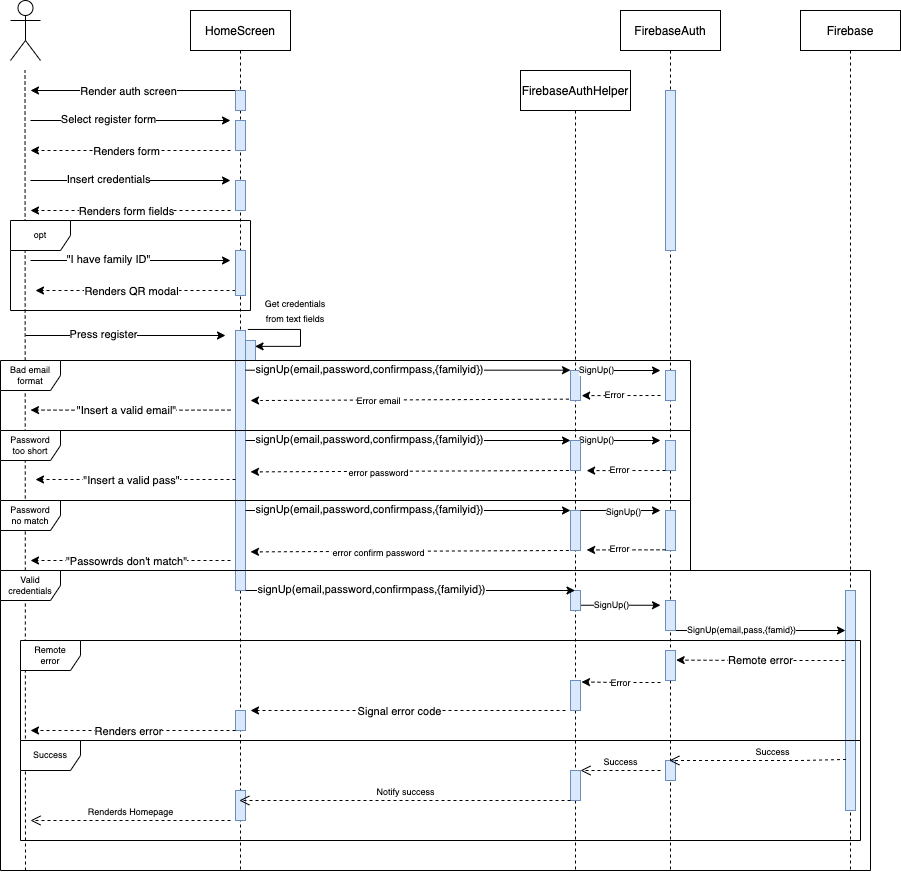
\includegraphics[scale=0.45]{./Images/runtime/sequence1.png}
  \caption{User signs up}
\end{figure}





\def\fillandplacepagenumber{%
 \par\pagestyle{empty}%
\vbox to 0pt{\vss}\vfill
\vbox to 0pt{\baselineskip0pt
   \hbox to\linewidth{\hss}%
   \setlength{\footskip}{70pt}
   \baselineskip\footskip
   \hbox to\linewidth{%
     \hfil\thepage\hfil}\vss}}

\begin{landscape}
\begin{figure}[h]
\vspace*{-2cm}
\noindent
\centering
\centerline{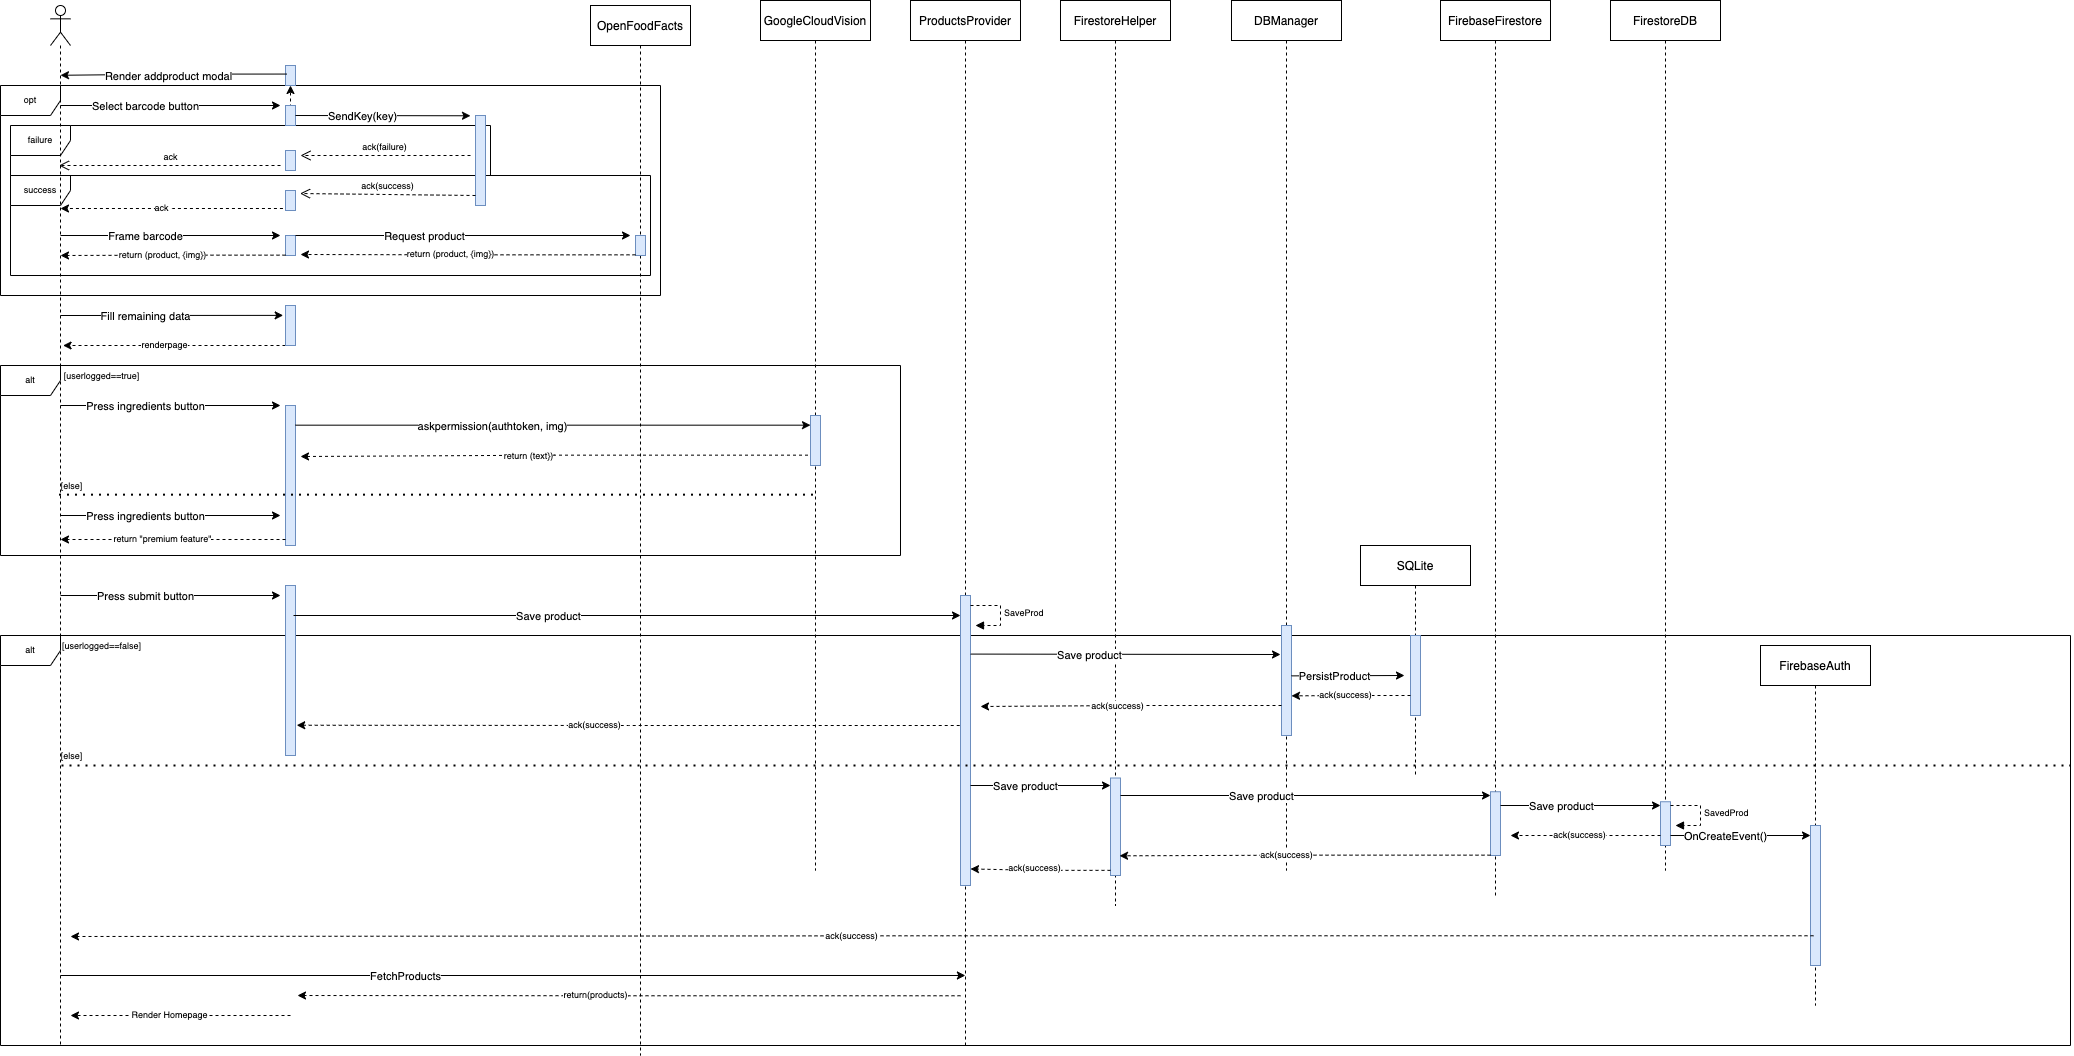
\includegraphics[scale = 0.37]{./Images/runtime/sequence2.png}}
\vspace*{-1cm}
    \caption{User adds a product}
    \vspace*{-12cm}
\end{figure}
\fillandplacepagenumber
\end{landscape}